\chapter{Approach}\label{approach}

\section{Overview}\label{sec:overview}

This chapter outlines the experimental methodologies and analyses conducted to investigate the challenges of length generalization in integer addition task. The primary focus is on understanding the limitations of absolute positional encodings and exploring methods to enhance the models' ability to generalize to longer sequences.

The initial experiments examine models trained with both absolute positional encodings and positional encodings focused on digit alignment, such as the Abacus encoding. Attention maps are analyzed to compare how these models process input sequences and to identify differences in digit alignment capabilities. Subsequent sections explore various data formatting techniques, including zero padding, reversing the answer, introducing random spaces, and employing a scratchpad approach. The impact of these techniques on length generalization is evaluated to determine if they can improve performance without altering the model architecture.

Further analysis investigates the effect of incorporating sub-task data—such as carry detection, digit-wise modular addition, reversing, and digit alignment—on the models' compositionality and length generalization capabilities. Experiments are conducted across different model dimensions and dataset sizes, comparing addition-only training with mixed-task training.

The chapter concludes with an examination of sub-task difficulty and learning order, highlighting how smaller models benefit more from sub-task learning. Mechanistic interpretability techniques are applied throughout to understand the internal mechanisms and failure modes of the models, providing insights into how positional encoding schemes affect generalization to longer sequences.


\section{Experimental Setup}\label{sec:experimental_setup}
This section details the experimental setup used to investigate the hypotheses outlined in Section~\ref{sec:research_questions}, including data formatting techniques, model configuration, training procedures, and evaluation metrics employed in the experiments. The experiments cover analysis of the effects of positional encodings, data formatting, and inclusion of sub-task data on the length generalization capabilities of transformer models in the multi-digit integer addition task.

\subsection{Data Formatting}\label{subsec:data_formatting}
Various data formatting techniques are employed and their effects on model generalization is exampined. All experiments use character-level tokenization; every character (digit, letter, symbol such as ``\texttt{+}'', ``\texttt{=}'', or space) is treated as an individual token. The vocabulary consists of 100 printable ASCII characters, ensuring that each token is represented uniquely. While character tokenization as such is a simple and flexible method, it is worth noting that current state-of-the-art LLMs use other subword tokenization schemes such as Byte-Pair Encoding (BPE) \parencite{sennrich_neural_2016,brown_language_2020}. Table~\ref{tab:data_formatting_examples} summarizes the different data formatting techniques with examples. Adding random spaces is particularly interesting as it applies a very simple and general idea to the integer addition problem and shows promise in improving length generalization.


\paragraph{Standard Format}
In the standard format, input sequences are represented as ``\verb|$a+b=c$|'', where $a$ and $b$ are the operands, and $c$ is the sum. The dollar signs ``\verb|$|'' denote the start and end of the sequence; the final ``\verb|$|'' also serves as the end-of-sequence token during autoregressive generation, stopping the process once it is generated. The plus ``\verb|+|'' and equals ``\verb|=|'' symbols separate the operands and the answer, respectively. For example, adding 123 and 456 is formatted as:
\begin{center}
    \verb|$123+456=579$|
\end{center}
This format serves as the baseline, with other formatting methods building upon it.

\paragraph{Zero Padding}
Zero padding involves aligning the digits by prepending operands and answers with leading zeros to match a fixed length $N_\text{pad}$. For instance, if $N_\text{pad}=5$, the addition of 123 and 456 becomes:
\begin{center}
    \verb|$00123+00456=00579$|
\end{center}
This method ensures that corresponding digits in different numbers always occupy the same absolute positions in the sequence, simplifying the learning of positional relationships. However, it does not actually solve the problem, since it requires prior knowledge of the maximum sequence length and can't be applied to sequences longer than $N_\text{pad}$.

\paragraph{Reversing}
Reversing the digits of operands and/or the answer switches the digit ordering to start with least significant digits, which follows the flow of operations like carry propogation. For example, reversing the operands yields:
\begin{center}
    \verb|$321+654=579$|
\end{center}
Reversing both operands and the answer gives:
\begin{center}
    \verb|$321+654=975$|
\end{center}
Reversing the operands alone, in principle, should not significantly impact performance, as the model can learn appropriate attention patterns to handle reversed sequences. However, reversing the answer theoretically simplifies the task by localizing carry propagation - since the model generates the output from left to right and can compute each digit independently instead of being forced to implicitly perform the carry propagation through the complete answer before generating the first answer digit.

\paragraph{Random Spaces}
Random spaces are inserted between symbols in the input sequence to disrupt fixed positional patterns and encourage the model to learn position-invariant representations. The number of spaces inserted is controlled by a parameter $\rho$, representing the maximum ratio of random spaces to non-space tokens in the operands. The maximum number of random spaces is calculated as $n_{\text{max}} = \rho \times L$, where $L$ is the length of the sequence (excluding the start token \texttt{\$}). The actual number of spaces $n$ is sampled uniformly from the set $\{0, \dots, n_{\text{max}}\}$. For example, if $\rho = 0.5$ and $L = 10$, then $n_{\text{max}} = 5$, and $n$ is randomly chosen from $\{0, 1, 2, 3, 4, 5\}$. The spaces are inserted at random positions within the operands. In all presented experiments, $\rho = 0.5$ when random spaces are enabled. An example of an input sequence with random spaces is:
\begin{center}
    \verb|$1 23 +4  5 6=579$|
\end{center}

\paragraph{Scratchpad}\label{par:scratchpad}
A scratchpad, or chain-of-thought, includes intermediate computational steps before the final answer, promoting step-by-step reasoning. This format also allows for the evaluation of intermediate results and aids in understanding the model's reasoning process. However, it requires task-specific data and therefore is not a general method. The scratchpad consists of reversed operands (reversing), modular addition with carry notation separated by semicolons (partials), and the final answer separated by a vertical bar. An example with comments describing the parts is given below (the line breaks are included for convenience and not part of the actual sequence):
\begin{center}
    \begin{tabular}{l l}
        \verb|$567+789=7 6 5 + 9 8 7;| & \textit{Input equation and reversed operands}             \\
        \verb|c=0,7+0+0=7,c=0;|        & \textit{Sum of units digit, no carry initially}           \\
        \verb|6+9+0=5,c=1;|            & \textit{Sum of tens digit, carry generated}               \\
        \verb|5+8+1=4,c=1;|            & \textit{Sum of hundreds digit and carry, carry generated} \\
        \verb|0+7+1=8,c=0|             & \textit{Sum of thousands digit and previous carry}        \\
        \texttt{|8457\$}               & \textit{Final result}
    \end{tabular}
\end{center}

This sequence represents the addition of 567 and 789 with detailed computation steps, where \texttt{c} denotes the carry variable.


\begin{table}[ht]
    \centering
    \caption{Examples of Data Formatting Techniques}
    \label{tab:data_formatting_examples}
    \begin{tabular}{ll}
        \toprule
        \textbf{Format}                                        & \textbf{Example}                                           \\
        \midrule
        Plain                                                  & \verb|$123+456=579$|                                       \\
        Zero Padding (to length 5)                             & \verb|$00123+00456=00579$|                                 \\
        Reversed Operands                                      & \verb|$321+654=579$|                                       \\
        Reversed Answer                                        & \verb|$123+456=975$|                                       \\
        Reversed Operands and Answer                           & \verb|$321+654=975$|                                       \\
        Random Spaces                                          & \verb|$12  3 +45 6=579$|                                   \\
        Scratchpad                                             & \begin{tabular}[t]{@{}l@{}} \verb|$567+789=7 6 5 + 9 8 7;| \\
                                                                     \verb|c=0,7+0+0=7,c=0;|                     \\
                                                                     \verb|6+9+0=5,c=1;|                         \\
                                                                     \verb|5+8+1=4,c=1;|                         \\
                                                                     \verb|0+7+1=8,c=0|                          \\
                                                                     \texttt{|8457\$}
                                                                 \end{tabular} \\
        Subtask Prefix (placeholder \texttt{xxx})\footnotemark & \verb|xxx$123+456=321+654$|                                \\
        \bottomrule
    \end{tabular}
\end{table}

\footnotetext{See Section~\ref{subsec:data_gen} for details on subtasks and corresponding prefixes.}


\subsection{Data Generation}\label{subsec:data_gen}

The training and test datasets for the experiments are systematically generated to evaluate the length generalization capabilities of transformer models on integer addition tasks. Each dataset consists of addition problems where both operands \( a \) and \( b \) are positive integers of equal number of digits, denoted as the \emph{digit length}. An addition problem involving operands of \( n \) digits is referred to as an \( n \)-digit or \( n \times n \) addition problem. For instance, a ``4-digit'' or ``4x4'' addition refers to both operands having exactly four digits.

Multiple datasets are created, each encompassing a specific range of in-distribution (ID) digit lengths for training and corresponding out-of-distribution (OOD) digit lengths for testing. The datasets are designed to assess the models' ability to generalize to sequence lengths beyond those seen during training. In each case, the datasets are split into training, validation, and test sets. The training set contains a specified number of ID digit length samples, while separate validation and test datasets are generated for ID and OOD digit lengths. To prevent data contamination, all samples in the validation and test sets are unique and not present in the training set.

The operand values are randomly sampled to ensure uniform coverage of possible combinations within the specified digit lengths. Numbers are generated such that they have exactly the specified number of digits (i.e., they do not start with zero). Unless specified otherwise, no attempt is made to balance the digit distribution nor the number of carries required in the addition operations across the samples.

Following the methodology of \cite{lee_teaching_2023}, for 1-digit operands (1x1 addition), all possible 100 combinations (operands ranging from 0 to 9) are included in the training dataset and therefore excluded from the test sets to avoid overlap. For 2-digit operands, 900 samples are randomly selected, and for 3-digit operands, 9000 samples are used. For digit lengths of 4 and above, an equal number of samples per digit length are randomly generated to fill the remaining training set size.

Out-of-distribution test sets are constructed by including digit lengths not present in the training data. Each OOD test set contains 1000 unique samples for each OOD digit length to evaluate the model's length generalization performance.

\paragraph{Sub-Task Data}

To enhance the compositional learning abilities of the models and investigate their impact on length generalization, various sub-task data was incorporated into some datasets. The sub-tasks include \emph{reversing}, \emph{carry detection}, \emph{digit-wise modular addition}, and \emph{digit alignment}. Each sub-task focuses on a specific aspect of the addition process, aiming to help the model learn underlying algorithmic components that could facilitate better generalization.

In contrast to the scratchpad approach, where intermediate computations are appended sequentially (leading to potential compounding errors), the sub-task training treats each sub-task as an independent auxiliary task. This method allows the model to learn each sub-task simultaneously without relying on the outputs of other tasks. Conversely, sub-task training implicitly involves composing multiple algorithmic parts due to pressure from the complete addition problem included alongside sub-tasks, instead of enforcing composition in each sequence.

To allow the model to differentiate between the sub-tasks each example includes a 3-letter task prefix, resulting in the format \texttt{xxx\$a+b=c\$}, where \texttt{xxx} denotes the sub-task identifier, and \texttt{c} represents the sub-task-specific output.

The sub-tasks, their prefixes, and their formats are as follows:

\begin{itemize}
    \item \textbf{Digit Alignment} (\texttt{ali}): Focuses on aligning the digits of the two operands for position-wise operations. The model learns to output the corresponding digit pairs from each operand.

          Example: \texttt{ali\$1234+4567=1+4,2+5,3+6,4+7\$}

    \item \textbf{Reversing} (\texttt{rev}): Involves reversing the digits of each operand. This sub-task helps the model understand the reversal operation, which inverts the propagation order from least significant digit to most.

          Example: \texttt{rev\$1234+4567=4321+7654\$}

    \item \textbf{Carry Detection} (\texttt{car}): Requires the model to identify positions where a carry operation would occur during addition. This sub-task is essentially a lookup operation from 2 digits to a binary value. The output is a string of ``c''s and dashes, indicating positions with and without carries respectively.

          Example: \texttt{car\$1234+4567=---c\$}

    \item \textbf{Digit-wise Modular Addition} (\texttt{mad}): The model performs addition modulo 10 on each pair of corresponding digits without considering carries. This sub-task is also in principle a lookup operation, from 2 digits to another digit.

          Example: \texttt{mad\$1234+4567=5791\$}

    \item \textbf{Addition} (\texttt{add}): The standard addition task, where the model computes the sum of the two operands. This serves as the main task and is included alongside sub-tasks in the dataset to facilitate composition of their output.

          Example: \texttt{add\$1234+4567=5801\$}
\end{itemize}

\paragraph{Datasets}

Several datasets were generated to support different experiments, each tailored to investigate specific aspects of length generalization and compositional learning. The datasets are described below:

\begin{itemize}
    \item \texttt{1-3\_digit}:
          \begin{itemize}
              \item \textbf{Training Set}: Contains 10,000 samples of addition problems where the operands have 1 and 3 digits. The dataset follows the methodology of \cite{lee_teaching_2023} and is used to replicate their baseline results.
              \item \textbf{Test Sets}: Separate test sets are created for each digit length from 1 to 4 digits, including OOD lengths of 2- and 4-digit addition problems not seen during training.
          \end{itemize}

    \item \texttt{1-7\_digit}:
          \begin{itemize}
              \item \textbf{Training Set}: Includes addition problems with operands ranging from 1 to 7 digits.
              \item \textbf{Test Sets}: Comprises test samples for digit lengths 1 to 8, with 8-digit addition serving as the OOD evaluation.
              \item \textbf{Purpose}: Replicates the extended baseline from \cite{lee_teaching_2023}, examining generalization to slightly longer sequences.
          \end{itemize}

    \item \texttt{generalize\_to\_longer}:
          \begin{itemize}
              \item \textbf{Training Set}: Consists of 1 million samples with digit lengths from 1 to 17 and 19 digits, intentionally excluding 18-digit problems to create an interpolation gap.
              \item \textbf{Test Sets}: Includes OOD test sets for 18-digit (interpolation) and 20-digit (extrapolation) addition problems.
              \item \textbf{Purpose}: Evaluates the model's ability to generalize to unseen lengths within (interpolation) and beyond (extrapolation) the training range.
          \end{itemize}

    \item \texttt{generalize\_to\_longer\_mini}:
          \begin{itemize}
              \item \textbf{Training Set}: Contains addition problems with digit lengths of 1 to 7 digits and 9 digits, deliberately omitting 8-digit problems.
              \item \textbf{Test Sets}: OOD test sets for 8-, 10-, and 11-digit addition problems.
              \item \textbf{Scales}: Training data is generated at multiple scales, with datasets of 10K, 100K, 1M, and 10M examples to study the impact of dataset size, where ``K'' denotes thousands and ``M'' denotes millions.
              \item \textbf{Purpose}: Investigates length generalization across different data scales and the effect of missing intermediate digit lengths.
          \end{itemize}

    \item \texttt{generalize\_to\_longer\_mini\_multitask}:
          \begin{itemize}
              \item \textbf{Composition}: Similar to \texttt{generalize\_to\_longer\_mini}, but includes all five sub-tasks (addition, reversing, carry detection, digit-wise modular addition, digit alignment) in the training data. Contains 2 variants for each scale: addition-only and multi-task training (including sub-tasks).
              \item \textbf{Scales}: Generated at the same data scales as above.
              \item \textbf{Purpose}: Examines the effect of sub-task training on compositionality and length generalization as compared to addition-only training.
          \end{itemize}
\end{itemize}

\subsection{Model Configuration}

Transformer decoder models are used as described in the Background chapter (Section~\ref{subsec:types_transformers}). Unless specified otherwise, a standard transformer decoder architecture is employed. The models are varied along several dimensions to assess their impact on performance:

\begin{itemize}
    \item \textbf{Number of layers (depth)}: The number of decoder layers.
    \item \textbf{Model dimension (width)}: The dimensionality of the model embeddings and hidden representations.
    \item \textbf{Number of attention heads}: The number of attention heads $h$ is chosen such that $d$ is divisible by $h$, commonly set to powers of 2.
    \item \textbf{Feed-forward layer dimension}: The hidden dimension of the feed-forward layers is set to $d_{\text{ff}} = 4 \times d$.
    \item \textbf{Context length}: The maximum input sequence length, denoted as $L_{\text{max}}$, is set based on the task requirements and is only relevant for models with absolute positional encodings.
\end{itemize}

Unless otherwise noted, models use absolute positional encodings. For experiments involving different positional encoding schemes, the specific configurations are detailed in the respective sections.

\subsection{Training and Evaluation}\label{subsec:training_evaluation}

\paragraph{Training Setup}
Overall, the training parameters from the NanoGPT \parencite{karpathy_nanogpt_2022} are used with modified number of steps, learning rates, and batch sizes. All models are trained using the AdamW optimizer with hyperparameters as shown in Table~\ref{tab:optimizer_hyperparameters}.

A learning rate scheduler with linear warm-up and cosine decay is used; for the first $T_{\text{w}} = 100$ iterations, the learning rate increases linearly from $0$ to the chosen learning rate. After warm-up, the learning rate at the current iteration $\eta(t)$ is cosine-annealed to a minimum learning rate of $\eta_{\text{min}} = 0.1 \times \eta$ over the course of training until maximum number of iteartions $T_{\text{max}}$ according to the formula:
\[
    \eta(t) =
    \begin{cases}
        \eta_{\text{max}} \times \dfrac{t}{T_{\text{w}}},                                                                                                                          & \text{if } t < T_{\text{w}}                        \\
        \eta_{\text{min}} + \dfrac{1}{2} (\eta_{\text{max}} - \eta_{\text{min}}) \left[1 + \cos\left( \pi \dfrac{t - T_{\text{w}}}{T_{\text{max}} - T_{\text{w}}} \right) \right], & \text{if } T_{\text{w}} \leq t \leq T_{\text{max}} \\
        \eta_{\text{min}},                                                                                                                                                         & \text{if } t > T_{\text{max}}
    \end{cases}
\]
where $t$ is the current iteration.

The batch size is selected based on the task, the model size and the sequence length to maximize GPU utilization while avoiding memory constraints. For large models or long sequences, gradient accumulation over multiple steps is employed to achieve an effective batch size. The number of training epochs is not set explicitly, rather the number of optimizer steps (iterations) is used. Answer loss masking (as described in Section~\ref{subsec:training_inference}) is applied during training unless specified otherwise. This means that the loss is computed only over the tokens corresponding to the answer part of the sequence, excluding any start tokens or padding tokens.

\begin{table}[h]
    \centering
    \caption{Optimizer Hyperparameters}
    \label{tab:optimizer_hyperparameters}
    \begin{tabular}{lcc}
        \toprule
        Hyperparameter & Value              \\
        \midrule
        Optimizer      & AdamW              \\
        Learning rate  & $3 \times 10^{-4}$ \\
        Betas          & $(0.9, 0.999)$     \\
        Epsilon        & $1 \times 10^{-8}$ \\
        Weight decay   & $0.1$              \\
        \bottomrule
    \end{tabular}
\end{table}


\paragraph{Inference Procedure}
During inference, top-$k$ sampling with $k=1$ is used, which corresponds to greedy decoding by selecting the token with the highest probability at each timestep. Although beam search was implemented and tested, it did not yield significant improvements due to the sharpness of the output distribution; the model's predictions are typically highly confident, with the softmax probabilities concentrated on a single token.

\paragraph{Evaluation Metrics}
For all experiments, the models are evaluated using two primary metrics:

\begin{itemize}
    \item \textbf{Cross-Entropy Loss}: Calculated over the answer tokens only, providing a measure of the model's average log-likelihood of the correct answer tokens. Lower loss values indicate better performance. The loss is also related to the \emph{perplexity} of the model, which is the exponential of the loss and is often used as a metric in language modeling tasks. The perplexity represents the average number of choices the model has for the next token, with lower values indicating better performance.
    \item \textbf{Accuracy}: Defined as the proportion of samples where all answer tokens are predicted correctly, also known as full match accuracy. A single incorrect digit in the answer results in the sample being marked as incorrect. To compute the accuracy, autoregressive inference (as described in Section~\ref{subsec:training_inference}) is used to generate the full answer sequence one token at a time until the end-of-sequence token is predicted or the maximum sequence length is reached. Higher accuracy values indicate better performance. The cross-entropy loss can be used to compare model performance when the accuracy is the same, e.g. when models have been trained short of full convergence and task accuracy is 0.
\end{itemize}

During training, both training and validation losses are recorded to monitor the learning dynamics. Models are evaluated on validation sets corresponding to both in-distribution (ID) and out-of-distribution (OOD) digit lengths to assess their generalization capabilities.


\section{Limitations of Absolute Positional Encoding}\label{sec:absolute_positional_limitations}

The limitations of absolute positional encoding become evident when evaluating length generalization in integer addition tasks. Models using absolute positional encodings are unable to generalize even to slightly longer sequences than those seen during training, failing to interpolate or extrapolate to unseen lengths. This failure appears to stem from the inability to extend learned attention patterns beyond the training lengths. Evidence from the analysis of the attention scores presented in Section~\ref{subsec:digit_alignment_pe} indicates that models with absolute positional encodings lack the sharp and well-formed attention patterns observed in models using positional encodings like the Abacus encoding. The absolute positional encoding struggles to precisely select the correct digits based on their positions, leading to misalignment in longer sequences. Introducing random spaces into the input sequences slightly smoothens the attention maps, which helps the model generalize in a limited way.

Furthermore, analysis of the next-token prediction uncertainty in Section~\ref{subsec:length_generalization_baseline} reveals that models exhibit high confidence in their predictions for in-distribution lengths but become increasingly uncertain for out-of-distribution lengths, especially for longer sequences. While for in-distribution digit positions the distribution over possible next tokens is usually collapsed, with all probability mass concentrated on the correct token. With OOD positions, on the other hand, next token distribution becomes more uniform and the probability of predicting the correct next token decreases towards zero. This suggests that extending the position addressing patterns to OOD lengths is the main issue, consistent with the literature indicating that vanilla Transformers struggle with index-based addressing operations.

By addressing the digit alignment problem, for example through the use of specialized positional encodings like the Abacus encoding \parencite{mcleish_transformers_2024}, models can generalize well to longer sequences without any other modifications. However, the challenge remains to enhance the generalization capabilities of models using standard absolute positional encodings without task-specific modifications. Introducing random spaces into the sequences is a potential strategy to encourage generalization, allowing models to interpolate and extrapolate to slightly longer sequences. The effects of different data formatting strategies, including the addition of random spaces, on length generalization are explored in the subsequent section. First, the baselines for length generalization are established demonstrating complete failure to generalize to any unseen lengths. Then, experiments are described that investigate the hypotheses that digit alignment is the root cause of failure and adding random spaces is a solution that partially address it while requiring no changes to the architecture.

\begin{figure}[!h]
    \centering
    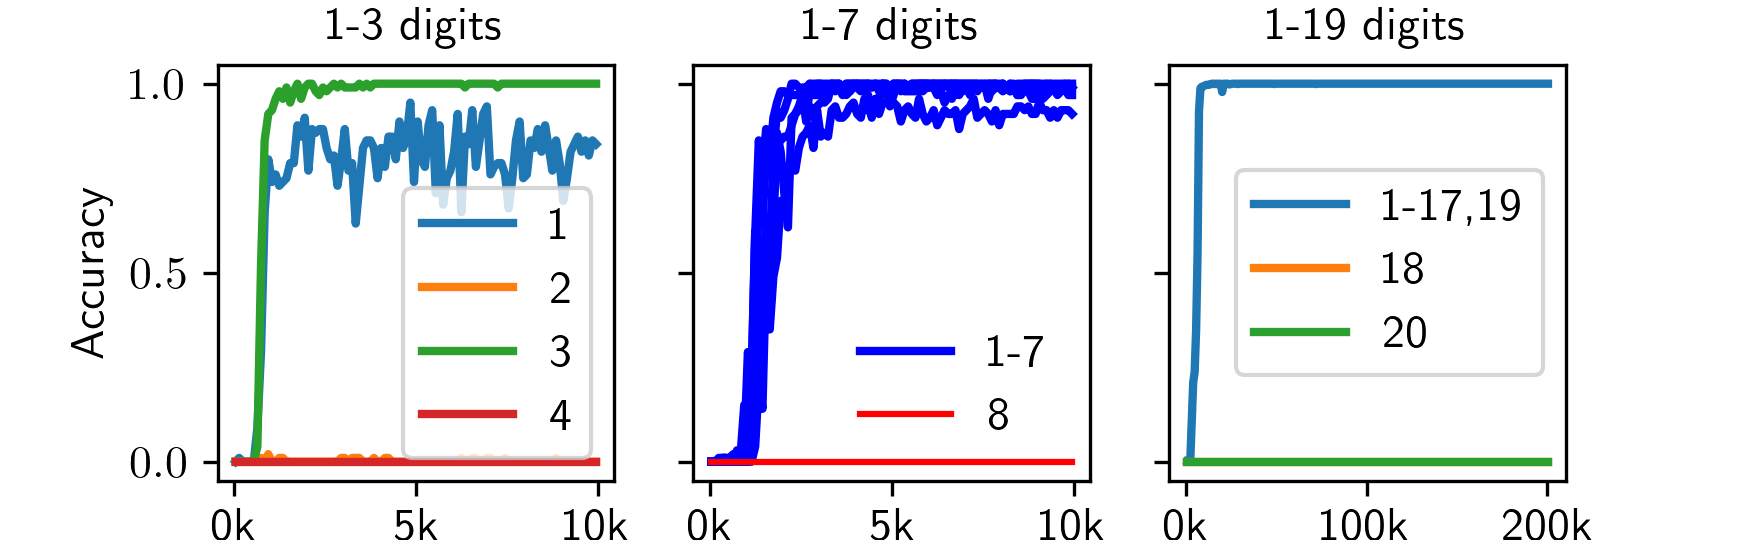
\includegraphics[width=\textwidth]{fig/baseline_and_longer.png}
    \caption{Baseline performance of Transformer decoder with absolute positional encodings over training. The model is a NanoGPT with 6 layers, 768 embedding dimension, and 4 attention heads. (Left) Model trained on 1 and 3-digit sequences fail to generalize to 2 and 4-digit sequences. (Middle) Same failure to generalize happens when trained on 1-7 digits and additionally tested on 8 digits. (Right) Model trained on 1--17 and 19-digit sequences fail to generalize to 18 and 20-digit sequences.}
    \label{fig:baseline_and_longer}
\end{figure}

\begin{figure}[!h]
    \centering
    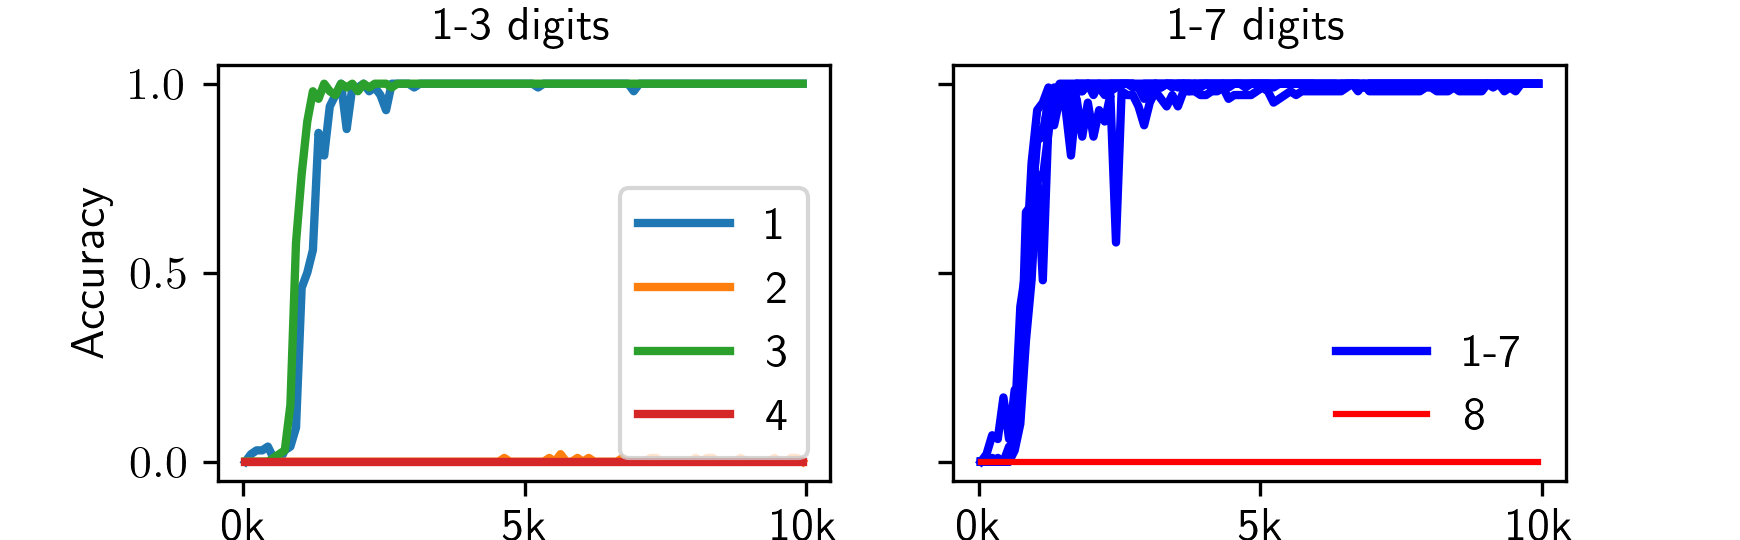
\includegraphics[width=0.9\textwidth]{fig/baseline_and_longer_ut.png}
    \caption{Baseline performance of Universal Transformer with absolute positional encodings over training. The model has embedding dimension of 384, 6 attention heads, and 3 recurrent steps (in encoder and decoder each). Similar failure to generalize is observed as in decoder-only model in Figure~\ref{fig:baseline_and_longer}.}
    \label{fig:baseline_and_longer_ut}
\end{figure}

\subsection{Length Generalization Baseline}\label{subsec:length_generalization_baseline}

To establish a baseline for length generalization, models with absolute positional encodings were trained on integer addition tasks with operands of certain digit lengths and tested on both seen and longer unseen digit lengths. Specifically, models were trained on sequences with operands of 1 and 3 digits and evaluated on sequences with operands of 2 and 4 digits. The models failed to generalize to the unseen lengths, demonstrating poor performance on both interpolation (lengths between those seen during training) and extrapolation (lengths beyond those seen during training). This inability to generalize supports the hypothesis that absolute positional encodings limit the model's capacity to handle sequences longer than those encountered during training.

In another experiment, models were trained on sequences of 1--7 digits and tested on sequences of 8 digits. The models again failed to generalize to the unseen lengths, further confirming the limitations of absolute positional encodings in facilitating length generalization for integer addition tasks.

\paragraph{Longer Training Sequences}
To investigate whether training on longer sequences could alleviate this issue, models were trained on sequences with operands of 1--17 and 19 digits and tested on sequences with operands of 18 and 20 digits. Despite the increased training sequence lengths, the models still failed to generalize to the unseen lengths in the vanilla setup with absolute positional encodings. This suggests that merely extending the training sequence lengths does not enable models with absolute positional encodings to generalize to longer sequences.

Figure~\ref{fig:baseline_and_longer} illustrates the performance of models trained under these configurations, showing that absolute positional encodings inherently limit the model's ability to generalize to unseen sequence lengths. Moreover, just making architectural changes such as using Universal Transformer (UT) does not solve the issue, as shown in Figure~\ref{fig:baseline_and_longer_ut}. The UT model also fails to generalize to unseen lengths, indicating that the problem is not specific to the decoder-only architecture.

\paragraph{Next-Token Uncertainty}
Analysis of the next-token prediction uncertainties provides further insights into the limitations of absolute positional encodings. For in-distribution lengths, models exhibit high confidence in their predictions, with low entropy in the next-token distributions. However, for OOD lengths, the models become increasingly uncertain, entropy of the next-token distributions increases, and the probability of the correct token decreases towards zero. Moreover, the analysis suggests that models often omit digits from different positions in the answer and thus attempt to end the sequence prematurely. This is in line with findings from \cite{newman_eos_2020} that the EOS token is output prematurely. Even if EOS token probability is suppressed to let the model output more digits in the answer, the digits are also often incorrect. Figure~\ref{fig:next_token_entropy} shows the average entropy and probabilities of the correct and end-of-sequence (EOS) tokens over the generated answer sequences for models trained on 1--17 and 19-digit lengths, demonstrating the contrast between in-distribution and OOD lengths; in distribution the model is confident and correct, and increasingly uncertain and incorrect for OOD lengths. This also shows that there is no attempt to extend the algorithm to OOD lengths, since instead of continuing to be confident (low entropy) but incorrect, the probabilities of next token actually degenerate into more diffuse distributions.

\begin{figure}[!h]
    \centering
    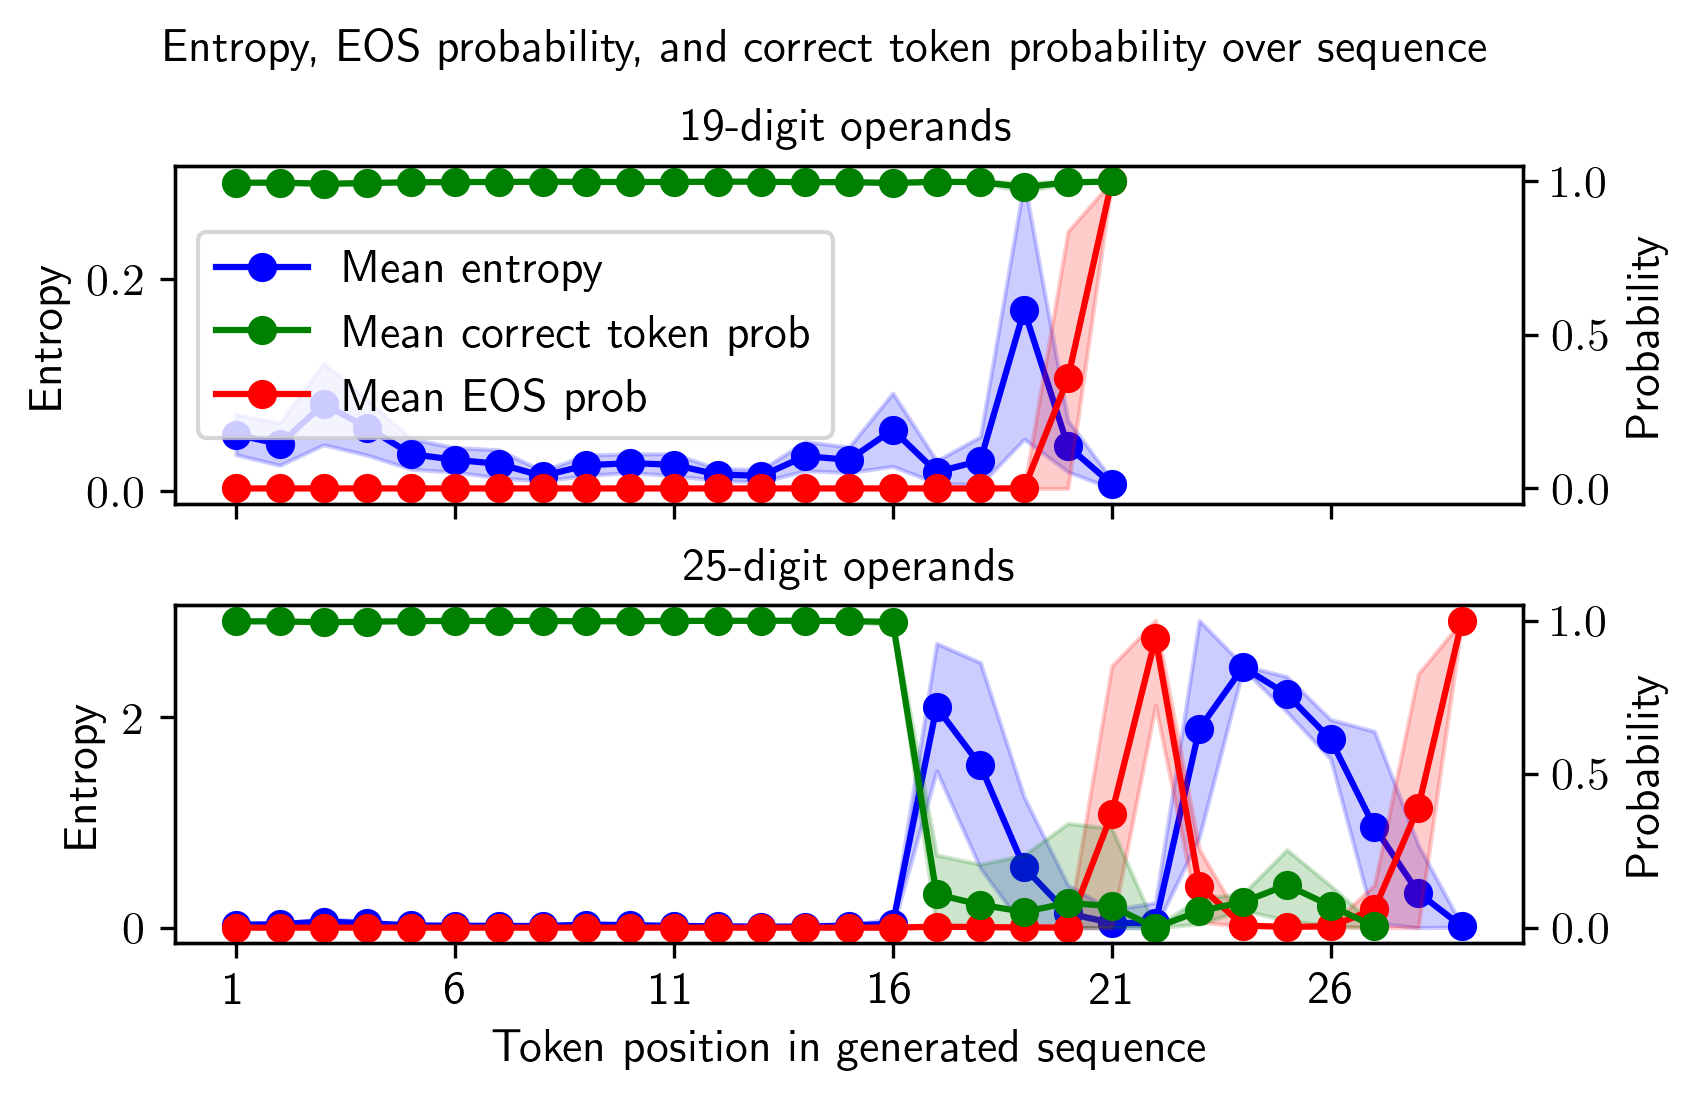
\includegraphics[width=0.9\textwidth]{fig/next_token_entropy.png}
    \caption{Next-token entropy analysis for a model trained on 1-17 and 19 digit lengths with random spaces. The blue, red, and green correspond to the mean entropy, mean probability of EOS token, and mean probability of the ground-truth answer token respectively, with shaded area showing the standard deviation over 100 different prompts. Top graph shows that for in-distribution lengths of up to 19, the entropy (uncertainty) of the next token is very low, and correct tokens are predicted. In the bottom graph, for 25 digit operands the absolute positions of the answer tokens after position 16 are already OOD, with more uncertainty and incorrect EOS prediction showing reliance on absolute positions. This is evidence that the learned algorithm is confident in distribution, but completely breaks down for out of distribution lengths.}
    \label{fig:next_token_entropy}
\end{figure}

\subsection{Positional Encodings Focused on Digit Alignment Improve Generalization}\label{subsec:digit_alignment_pe}

The inability of models with absolute positional encodings to generalize to longer sequences suggests that digit alignment is the root issue. To investigate this hypothesis, models were trained using both absolute positional encodings and positional encodings focused on digit alignment, such as the Abacus encoding, under the same setup. Specifically, models were trained on 100,000 samples with operand lengths of 1--7 digits and tested on OOD lengths of 8 and 10 digits.

\begin{figure}[!h]
    \centering
    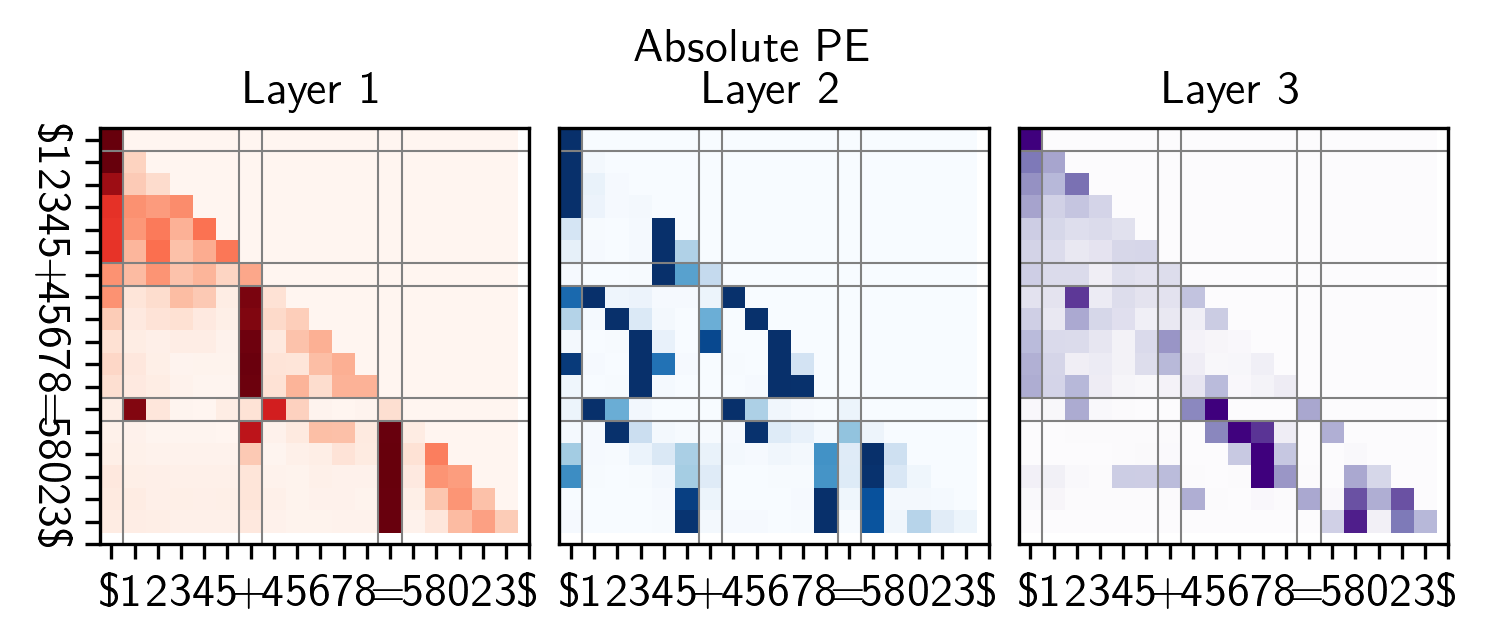
\includegraphics[width=0.8\textwidth]{fig/attn_map_abs_pe.png}
    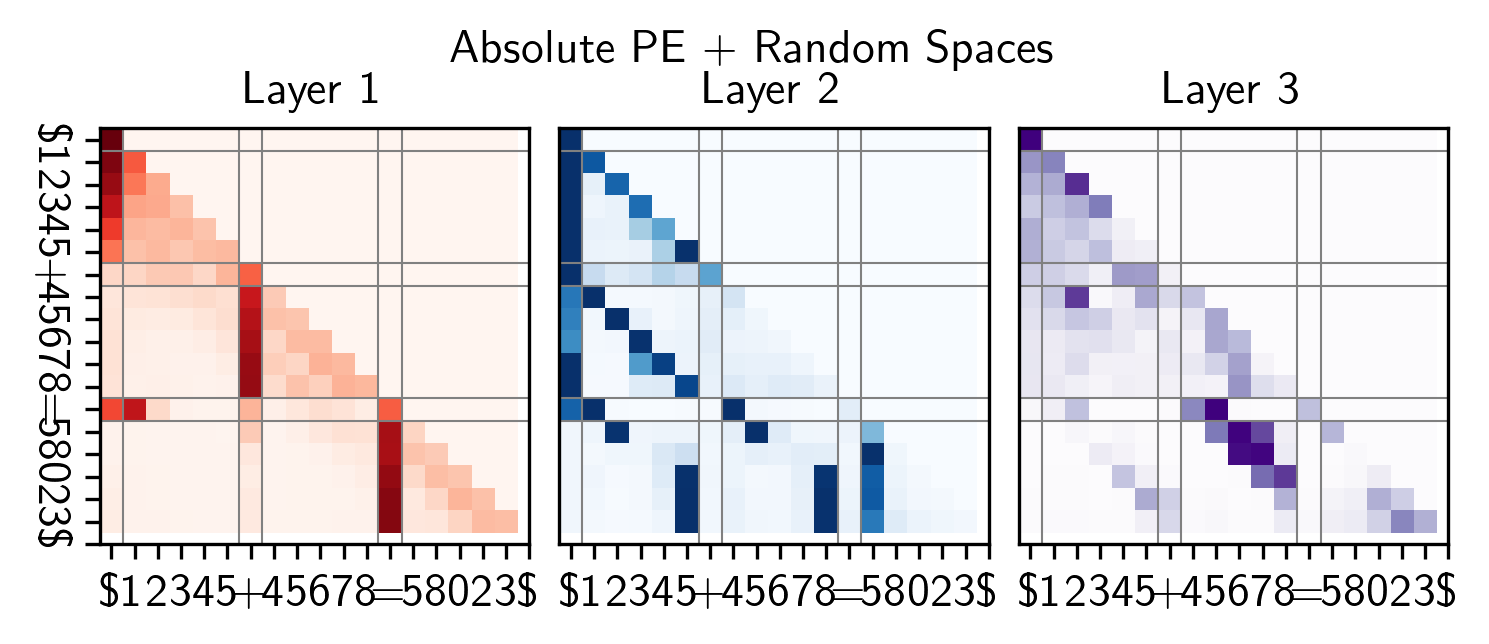
\includegraphics[width=0.8\textwidth]{fig/attn_map_abs_pe_random_spaces.png}
    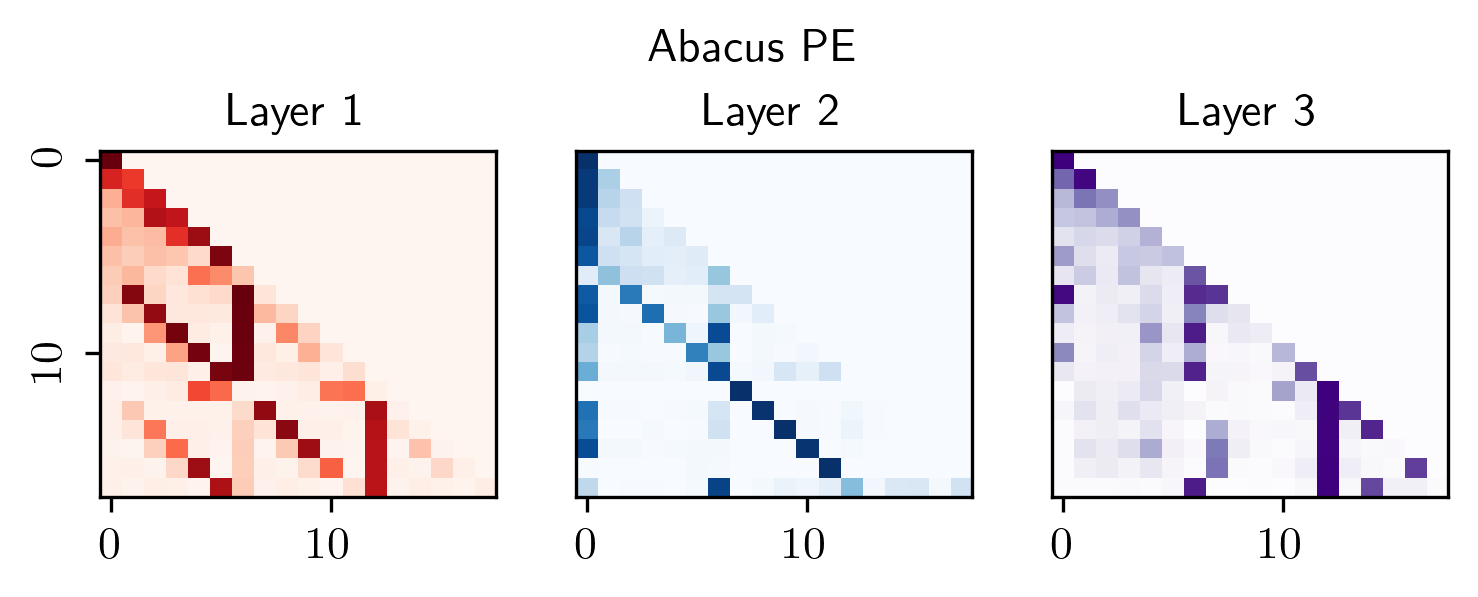
\includegraphics[width=0.8\textwidth]{fig/attn_map_abacus_pe.png}
    \caption{Comparison of attention maps (maximum over the 4 heads, after softmax) for models with (top) absolute positional encoding, (middle) absolute positional encoding with random spaces, and (bottom) Abacus positional encoding~\parencite{mcleish_transformers_2024}. The y and x axes are the target and source sequence, which are the same for the decoder-only model, color intensity shows how much a given target token ``attends'' to a source token. It is desirable to see orderly lines, since operations are done digit-wise and can be applied to longer sequences. The model with absolute positional encodings shows unclear attention patterns with some randomness, while the Abacus model is significantly less noisy. While random spaces do not fix the issue completely, the attention patterns are significantly more aligned. The differences are especially evident in Layer 2.}
    \label{fig:digit_align_attn_maps}
\end{figure}

Attention maps from these models reveal significant differences in how they process input sequences. Models with absolute positional encodings exhibit unclear and diffuse attention patterns that do not extend coherently to longer sequences. In contrast, models using the Abacus positional encoding display clearer attention maps, selecting the correct digits based on their positions, even for sequences longer than those seen during training.

Figure~\ref{fig:digit_align_attn_maps} illustrates the attention maps for the different models. The attention patterns in the Abacus model suggest that aligning digits effectively is crucial for generalizing integer addition to longer sequences. This supports the hypothesis that positional encodings focused on digit alignment enhance the model's capacity to generalize by facilitating correct digit alignment.

Furthermore, evaluation results, as shown in Figure~\ref{fig:pe_results}, demonstrate that models with positional encodings focused on digit alignment significantly outperform those with absolute positional encodings on OOD lengths. This underscores the importance of digit alignment in achieving length generalization in integer addition tasks.

\begin{figure}[!h]
    \centering
    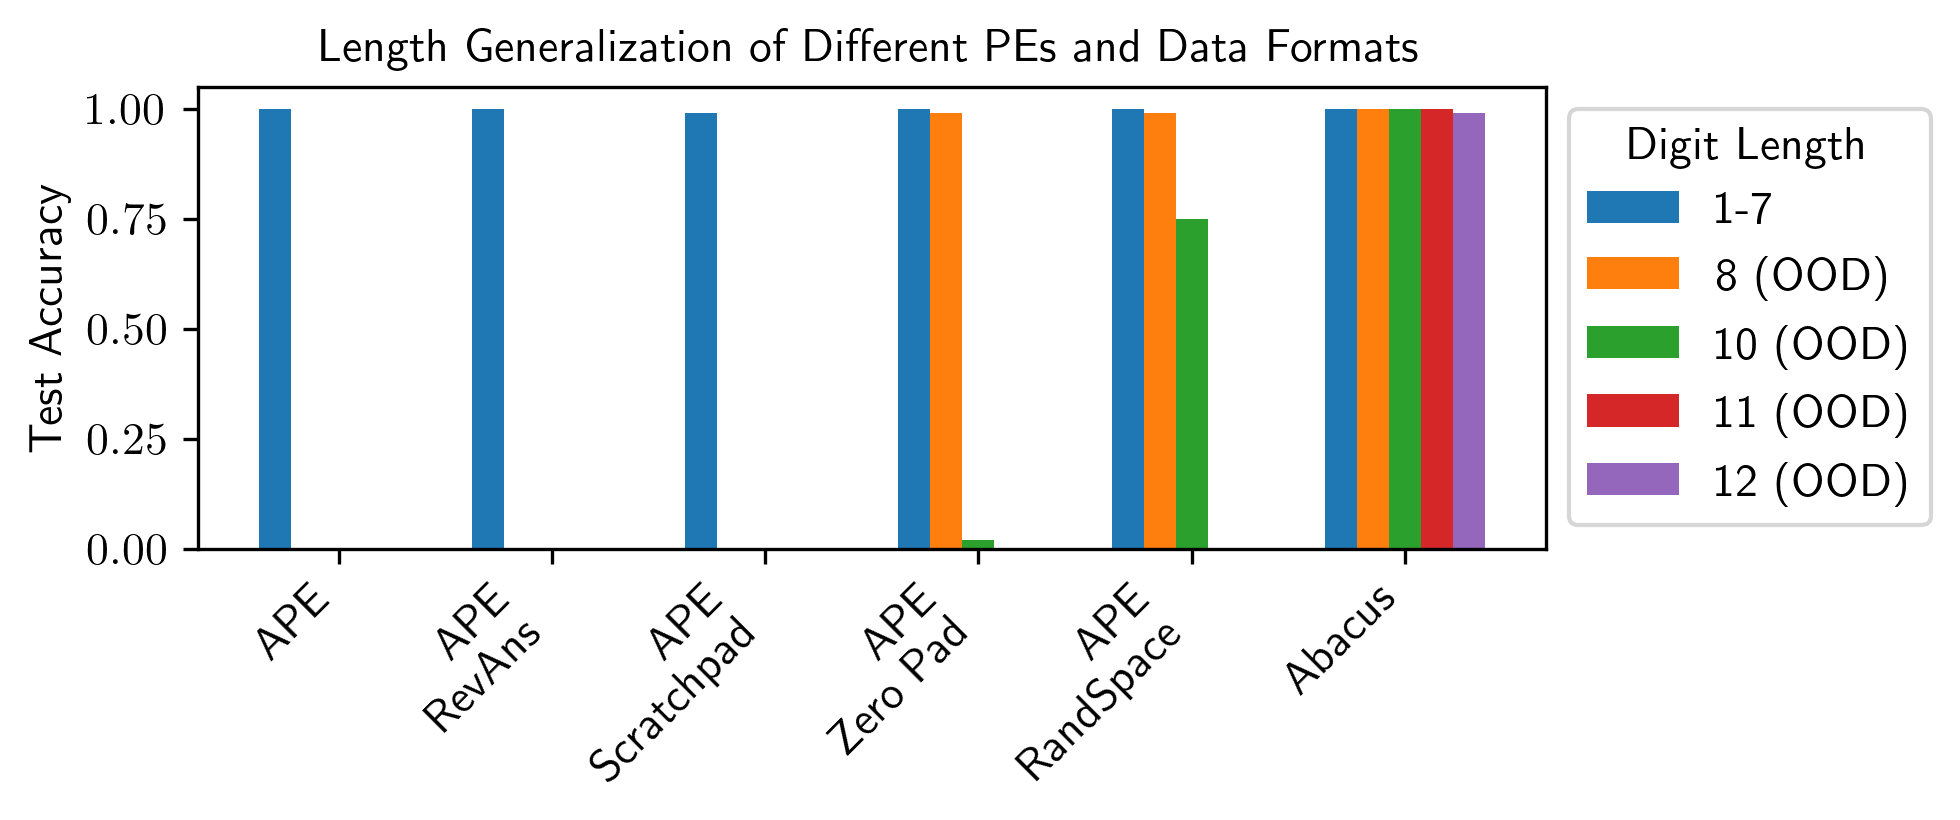
\includegraphics[width=0.9\textwidth]{fig/pe_results.png}
    \caption{Performance comparison of models with different positional encodings and data formatting methods on in-distribution (1--7 digits) and out-of-distribution (8, 10, 11, and 12 digits) lengths. Regular absolute positional encoding (APE) fails on all OOD lengths. Reversing the answer and scratchpad do not improve OOD accuracy. Zero-padding numbers to 13 digits improves interpolation (8-digit OOD length) but does not help extrapolation, while adding random spaces helps to partially extrapolate by one digit. Abacus encoding solves the underlying position alignment issue and generalizes to OOD lengths.}
    \label{fig:pe_results}
\end{figure}

\subsection{Breaking Positional Patterns in Absolute Positional Encodings Allows Weak Generalization}

To attempt to improve length generalization without altering the model architecture or introducing task-specific modifications, the impact of randomly adding spaces into input sequences was investigated. The hypothesis is that random spaces disrupt fixed positional patterns that the model might overfit to, encouraging it to learn more robust representations that are less dependent on absolute positions.

Experiments were conducted where random spaces were added to the input sequences during training according to the method described in Section~\ref{subsec:data_formatting}. The models trained with this data formatting strategy exhibited marginal improvements in length generalization, successfully interpolating to lengths within the training distribution and extrapolating to sequences that are one digit longer than those seen during training.

Attention maps of these models, as shown in Figure~\ref{fig:digit_align_attn_maps}, indicate that introducing random spaces smoothens the attention patterns, helping the model to generalize slightly better. The models become less reliant on fixed positional patterns and more capable of handling variations in the input sequences.

Evaluation results in Figure~\ref{fig:pe_results} compare the performance of models with absolute positional encodings, with and without random spaces, highlighting the modest gains in generalization achieved through this data formatting strategy.

\section{Impact of Other Data Formats on Length Generalization}\label{sec:other_data_formats_length_generalization}

Different data formatting strategies can influence the model's ability to generalize to longer sequences. This section investigates the effects of various data formatting techniques, including zero padding, reversing the answer or operands, introducing random spaces, and using a scratchpad approach, on length generalization in integer addition tasks.

\subsection{Zero Padding}

Zero padding involves padding the operands to a fixed maximum length by adding leading zeros, effectively aligning the digits of the operands. This technique directly addresses the digit alignment issue by ensuring that digits in the same positional place are aligned across all sequences.

Experiments were conducted where models were trained on zero-padded sequences up to a fixed maximum length. The results showed that zero padding significantly improved performance on sequences up to the maximum padded length, as the model could effectively learn to align and process the digits.

However, zero padding has inherent limitations. It requires prior knowledge of the maximum sequence length, which may not be practical in scenarios where the sequence lengths are unbounded or variable. Additionally, zero padding does not enable the model to generalize to sequences longer than the maximum padded length, as the model has not learned to handle sequences of greater length.

As shown in Figure~\ref{fig:pe_results}, zero padding improves performance on sequences up to the maximum padded length but does not help the model generalize to longer sequences beyond that length.

\subsection{Reversing the Answer}

Reversing the answer involves reversing the order of the digits in the output sequence. Theoretically, reversing the answer can simplify the addition task for the model by reducing the need for carry propagation through the entire answer before outputting the first digit. This is because the least significant digit, which is computed first in the addition process, becomes the first digit in the output sequence.

Experiments were conducted to assess the impact of reversing the answer on model generalization. Models were trained with and without reversed answers using absolute positional encodings. Contrary to expectations, reversing the answer did not lead to significant improvements in generalization performance. As shown in Figure~\ref{fig:pe_results}, the performance of models with reversed answers was comparable to those without reversal, even though reversing the answer conceptually simplifies the task.

Interestingly, during training, models with both reversed and non-reversed answers exhibited similar learning patterns. Initially, the models correctly predicted the most significant digits, gradually improving their predictions for the less significant digits as training progressed, up to the maximum in-distribution length. This phenomenon is shown in Appendix~\ref{app:additional_results}.

\subsection{Scratchpad}

The scratchpad approach involves including intermediate computation steps in the training data, similar to a chain-of-thought, where the model outputs not only the final answer but also the intermediate results leading to it. This method aims to make the underlying computation process explicit, potentially aiding the model in learning the algorithmic steps required for addition.

Experiments were conducted to evaluate the effectiveness of the scratchpad approach in improving length generalization. The results indicated that the scratchpad approach did not significantly enhance generalization to longer sequences. Models trained with scratchpad data exhibited similar performance on OOD lengths compared to models trained without it.

However, the scratchpad approach proved useful for mistake analysis. By examining the model's intermediate outputs, it was possible to identify specific points of failure in the computation process. This provided insights into which parts of the addition algorithm the model struggled with, such as carry propagation or digit-wise addition.

The limited effectiveness of the scratchpad approach in improving generalization contrasts with findings in the literature, where scratchpad has been shown to aid in generalization~\parencite{lee_teaching_2023}. One possible explanation is that smaller models, as used in these experiments, may not have sufficient capacity to leverage the additional information provided by the scratchpad like in the aforementioned paper. Figure~\ref{fig:scratchpad_eval} presents the evaluation results for the scratchpad approach, with violin plots of accuracy and edit distance by intermediate computation steps, showing which intermediate steps are most error-prone.

\begin{figure}[!h]
    \centering
    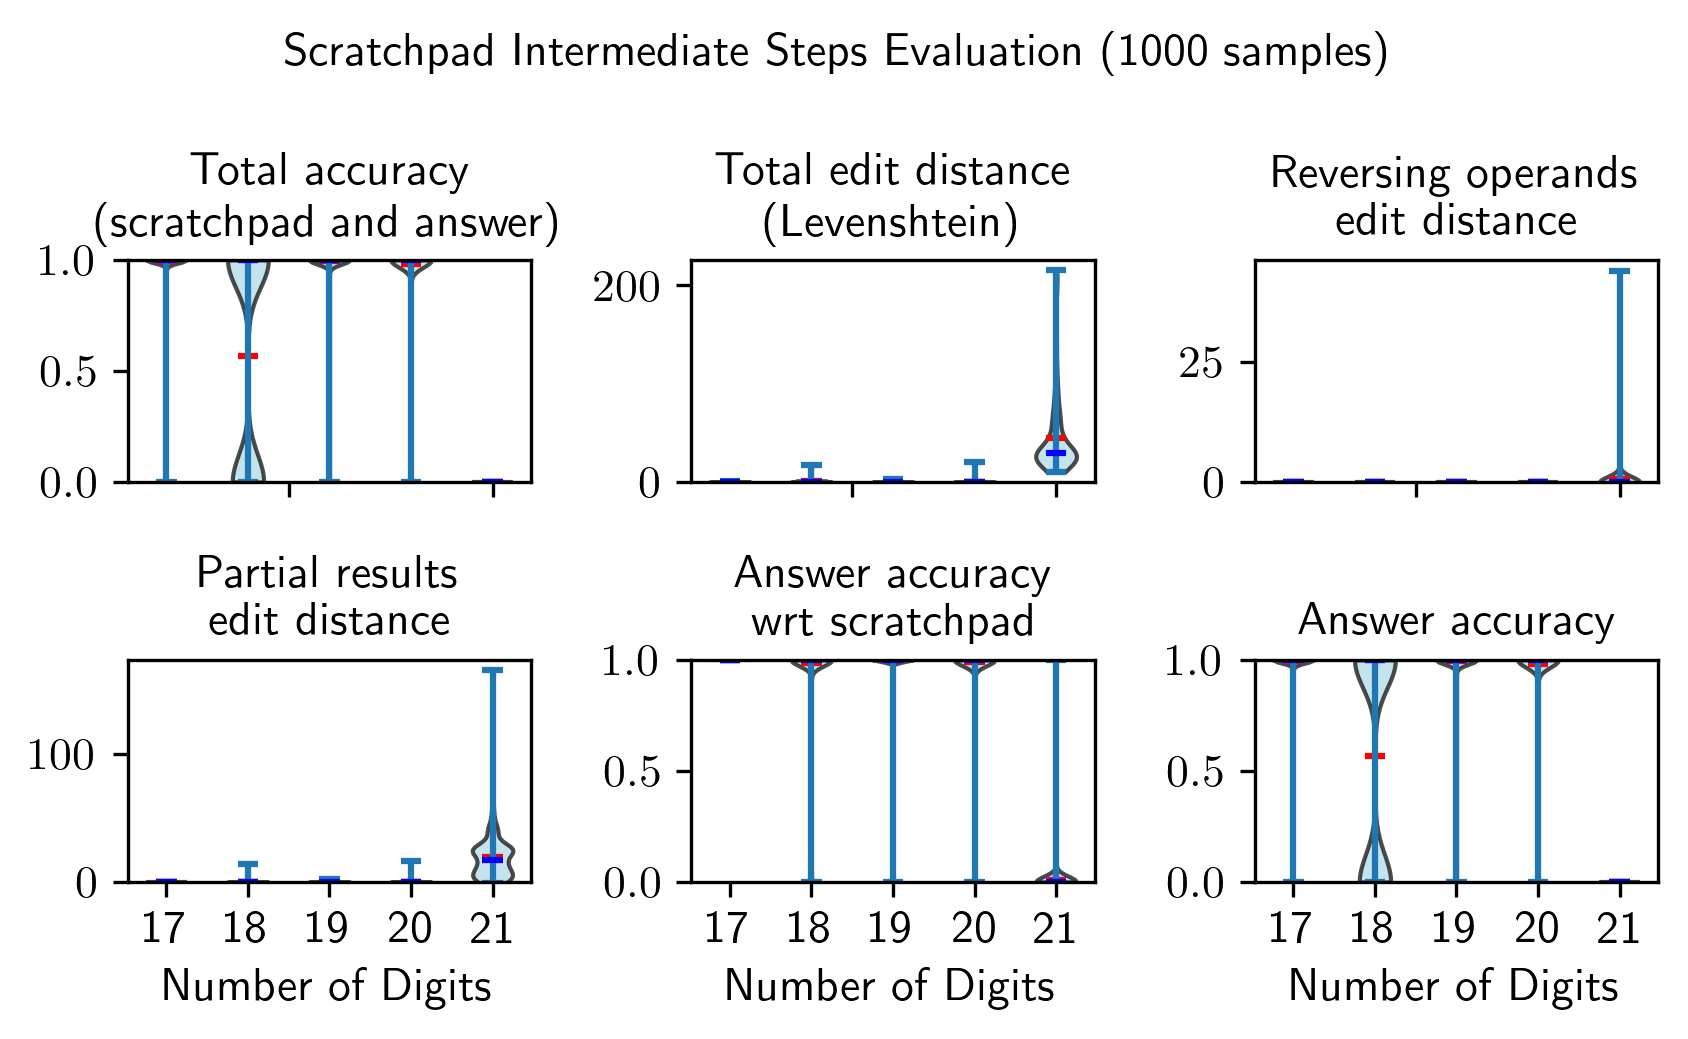
\includegraphics[width=0.9\textwidth]{fig/scratchpad_eval.png}
    \caption{Evaluation results for a model trained with scratchpad on 1-17 and 19 digits. The parts of the scratchpad format are described in Section~\ref{par:scratchpad}. The violin plots depict the distribution of accuracies and edit distances by intermediate steps. Most notably, for 18 and 20 digits OOD lengths, the accuracy of the answer with respect to scratchpad is very high (center bottom), and thus the main source of mistakes is performing the intermediate calculations and not ``reading off'' the answer, further hinting at the problem of digit alignment.}
    \label{fig:scratchpad_eval}
\end{figure}

Overall, while the scratchpad approach did not enhance length generalization, it provided insights into the model's internal computations and error patterns. The practicality of the scratchpad method is limited for tasks where intermediate computations are not readily available or known in practice.

\section{Sub-task Learning for Compositionality}\label{sec:subtask_learning}

Incorporating sub-task data into the training process aims to enhance the model's compositionality and length generalization capabilities by explicitly teaching the underlying algorithmic components of integer addition. This section explores the hypothesis that training on sub-tasks, such as carry detection, digit-wise modular addition, reversing, and digit alignment, can improve the model's ability to compose these functions and generalize to sequences longer than those seen during training.

\paragraph{Experimental Setup}
A comprehensive analysis was conducted across various model dimensions, ranging from 64 to 1536, and training dataset sizes of 10,000, 100,000, 1 million, and 10 million examples. Models were trained under two settings: addition-only and multi-task training, where the latter involved mixing addition tasks with sub-task data while matching the total number of samples. In all cases, the model is a decoder-only transformer with 6 layers and 8 attention heads, with absolute positional encodings and random spaces in the input sequences (ratio of random spaces to prompt length $\rho = 0.5$), optimizer and learning rate scheduler as described in Section~\ref{subsec:training_evaluation}.

The performance was evaluated over a range of different model widths due to the confounding phenomenon of \emph{deep double descent}, where increasing model capacity or training duration can initially lead to worse generalization before ultimately improving it. This was initially believed to challenge the traditional bias-variance tradeoff, where increasing model complexity was believed to always result in overfitting \parencite{belkin_reconciling_2019, nakkiran_deep_2021}. Deep double descent arises when models, especially overparameterized ones, first memorize the training data, but later discover more generalizable features, leading to improved performance on the test set and zero training loss. This phenomenon is still relevant in integer addition tasks, since the interpolation threshold — the point where the model transitions from memorization to generalization might change with respect to model and dataset size.

The main finding is that mixed-task training sometimes improves OOD loss, with the effect being particularly pronounced for smaller models and smaller dataset sizes. Moreover, in mixed-task settings smaller models exhibit a Pareto improvement in OOD loss without an increase in in-distribution loss, suggesting that sub-task learning can help the model learn more generalizable representations and algorithms. Interestingly, the double descent phenomenon is not observed in the experiments, as the loss does not visibly drop with larger models, indicating that either the covered size range is not sufficient to see the full effect, or the scaling behavior is fundamentally different for this algorithmic task.

\begin{table}[!h]
    \centering
    \caption{Comparison of OOD accuracy (in percentage) for models trained with addition-only and sub-task training across dataset sizes. Smaller datasets show greater improvement with mixed-task training. Despite weak absolute performance, sub-task training can marginally improve length generalization.}
    \label{tab:subtask_results}
    \begin{tabular}{lcccc}
        % \toprule
                    & \multicolumn{2}{c}{8 Digits} & \multicolumn{2}{c}{10 Digits}                             \\
        Dataset     & Acc (Add)                    & Acc (Mix)                     & Acc (Add) & Acc (Mix)     \\
        \midrule
        10K         & 7.0 ± 22.7                   & 35.4 ± 39.6                   & 0 ± 0     & 2.4 ± 8.4     \\
        100K        & 21.5 ± 29.7                  & 41.8 ± 36.5                   & 0 ± 0     & 1.0 ± 5.2     \\
        1M          & 16.1 ± 24.8                  & 39.5 ± 36.3                   & 0 ± 0     & 1.5 ± 7.6     \\
        10M         & 18.6 ± 33.1                  & 37.3 ± 37.2                   & 0 ± 0     & 3.1 ± 10.1    \\
        \midrule
        Improvement &                              & \textbf{+22.7}                &           & \textbf{+2.0} \\
        \bottomrule
    \end{tabular}
\end{table}

\subsection{Sub-Tasks Marginally Improve Length Generalization}

To evaluate the impact of sub-task learning on length generalization, models were trained under two settings: addition-only and mixed-task training. The mixed-task training involved combining the main addition task with various sub-tasks, such as carry detection, digit-wise modular addition, reversing, and digit alignment. The experiments spanned a range of model dimensions (from 64 to 1536) and dataset sizes (10,000 to 10 million examples).

The results indicate that incorporating sub-task data marginally improves length generalization, particularly for smaller models and smaller dataset sizes. As shown in Figure~\ref{fig:exp_27_val_loss_vs_n_embd}, smaller models (e.g., with a dimension of 64 and 8 attention heads) benefit more from mixed-task training compared to larger models. The smaller models exhibit lower OOD validation losses when trained with sub-tasks, suggesting that they are better able to leverage the compositional learning provided by the sub-tasks.

\begin{figure}[!h]
    \centering
    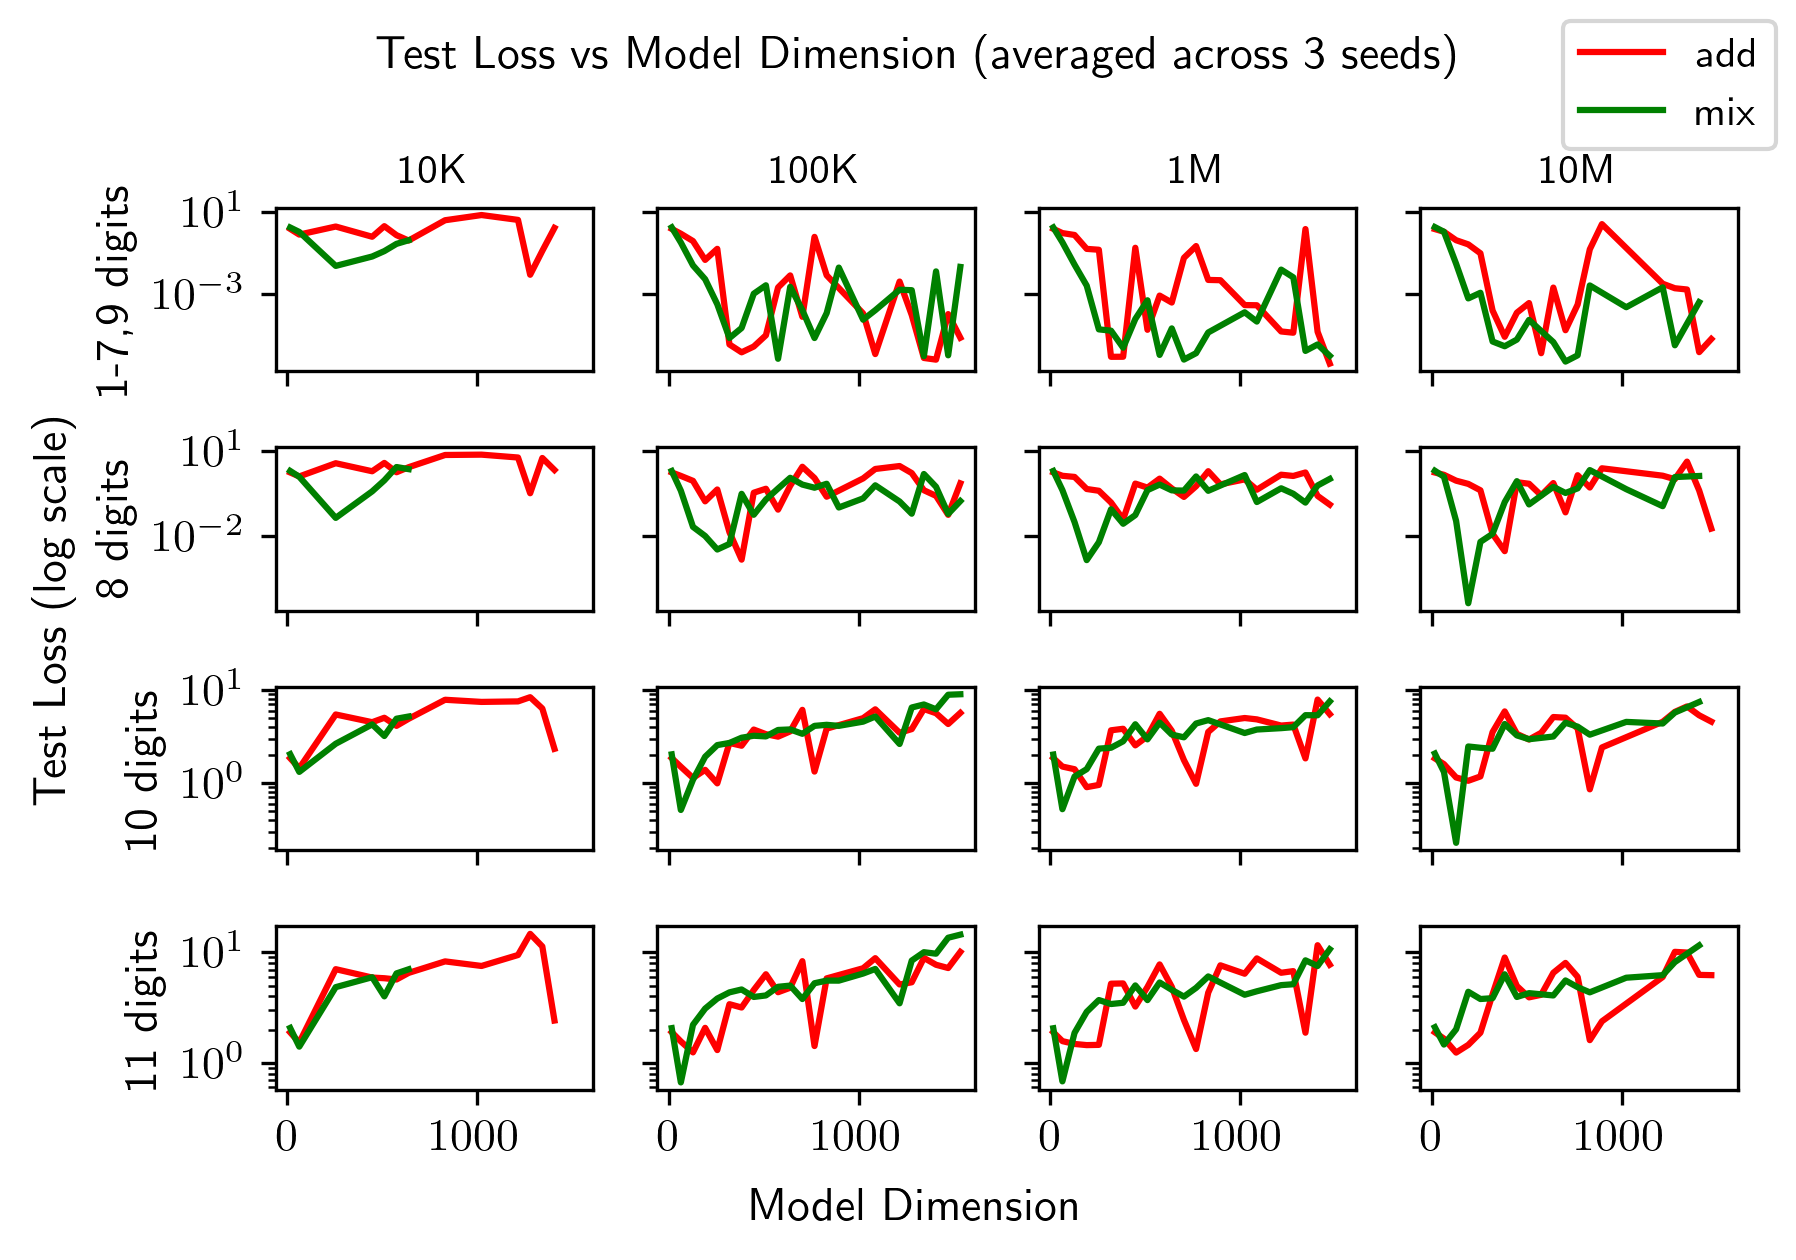
\includegraphics[width=\textwidth]{fig/exp_27_val_loss_vs_n_embd.png}
    \caption{Validation loss versus model dimension for addition-only (red) and multi-task training (green). The x axis corresponds to different model widths (embedding dimension). The effect of multi-task training is more pronounced in smaller models and diminishes as model size increases.}
    \label{fig:exp_27_val_loss_vs_n_embd}
\end{figure}

One possible explanation for this observation that smaller models improve more from subtask data is that larger models have sufficient capacity to memorize the training data, including the sub-tasks, without necessarily learning the underlying algorithms that facilitate generalization. In contrast, smaller models are constrained by their limited capacity and are thus compelled to learn more generalizable representations and algorithms, with the sub-tasks aiding in this process. Table~\ref{tab:subtask_results} summarizes the performance differences between addition-only and mixed-task training across different model dimensions and dataset sizes. The difference is positive in all cases with larger improvements observed in smaller models and datasets. Figure~\ref{fig:exp_27_val_loss_vs_n_embd} illustrates the validation loss versus model dimension for both in-distribution and OOD lengths, highlighting how mixed-task training can improve out-of-distribution performance, especially for smaller models.

Additionally, analyzing the in-distribution versus out-of-distribution losses reveals that in some cases, sub-task learning helps mitigate overfitting. As depicted in Figure~\ref{fig:subtask_overfitting}, smaller models (embedding dimension 64) achieve a Pareto improvement in OOD loss without an increase in in-distribution loss when trained with sub-tasks.

\begin{figure}[htb!]
    \centering
    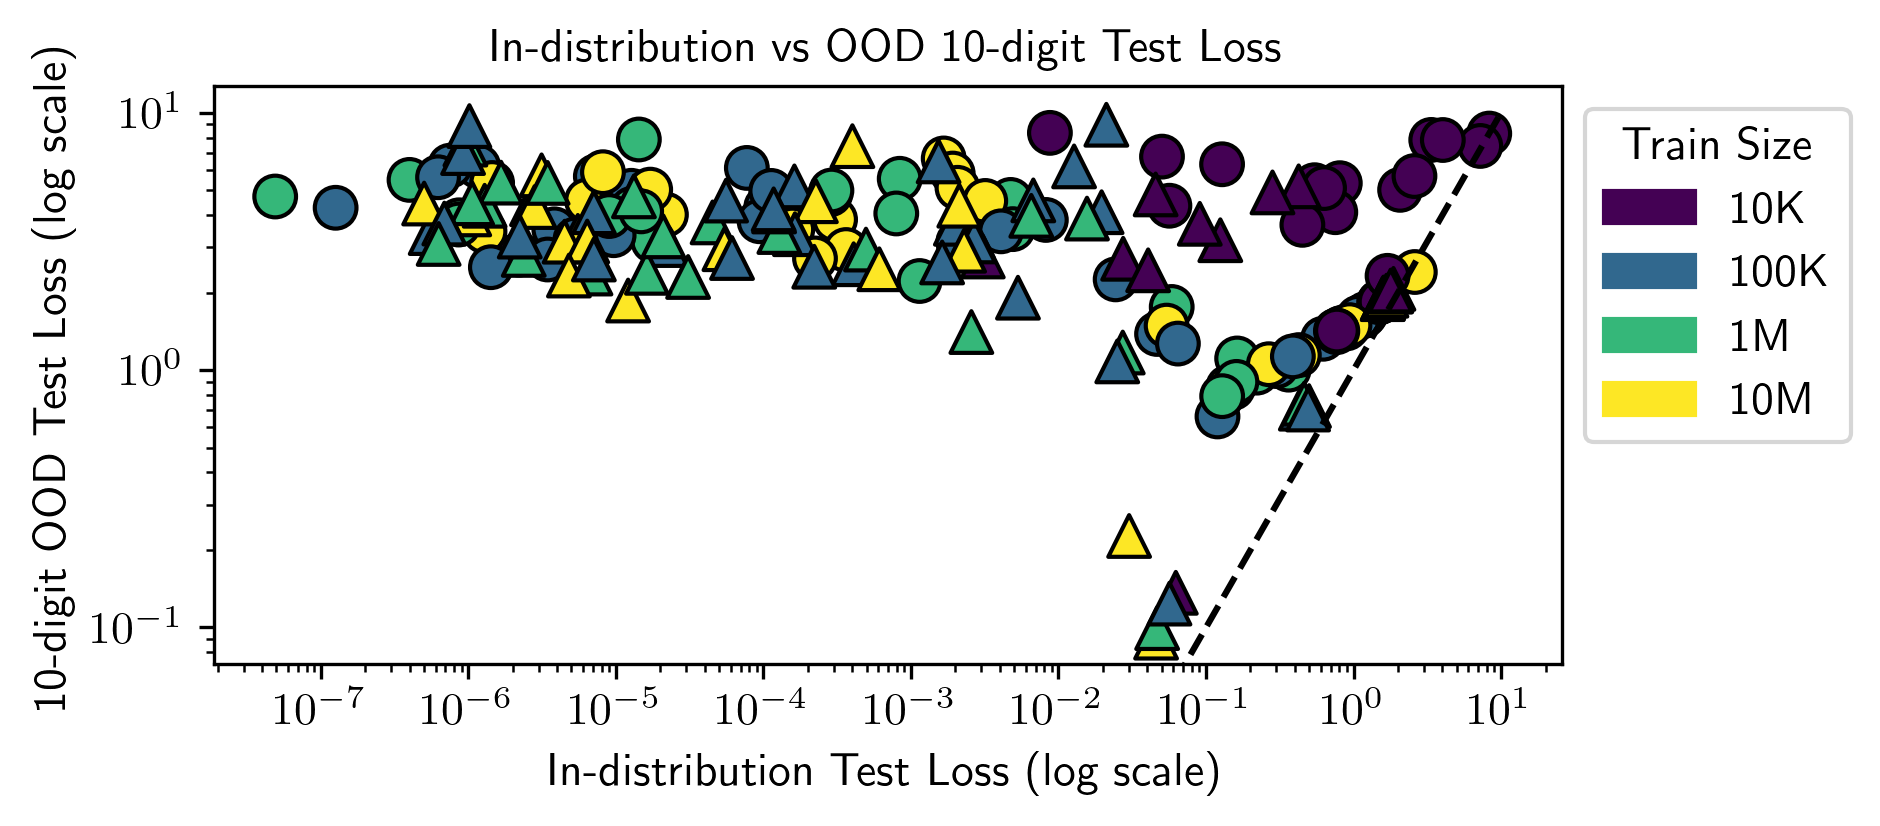
\includegraphics[width=0.9\textwidth]{fig/subtask_overfitting.png}
    \caption{Comparison of in-distribution test loss and 10-digit out-of-distribution (OOD) test loss across different training sizes for models trained on addition only (circles) and sub-tasks (triangles). Colors represent the training dataset size (10K, 100K, 1M, and 10M), and the dashed line indicates the diagonal where in-distribution and OOD losses match. Models trained with sub-tasks can achieve a lower OOD loss by an order of magnitude compared to addition-only training.}
    \label{fig:subtask_overfitting}
\end{figure}

\subsection{Smaller Models Benefit More from Sub-Tasks}

The experiments demonstrate that smaller models benefit more significantly from sub-task learning compared to larger models. Specifically, models with smaller dimensions exhibit greater reductions in OOD validation loss when trained with mixed tasks.

For the smallest model configuration (64 dimensions), the incorporation of sub-task data leads to a notable improvement in length generalization. In contrast, larger models (e.g., with 1536 dimensions) show minimal differences in performance between addition-only and mixed-task training. This suggests that larger models may already have sufficient capacity to memorize the training data, including the addition task, without relying on compositional learning provided by the sub-tasks.

The observed trend indicates that sub-task learning is particularly advantageous for models with limited capacity, as it encourages the learning of generalizable algorithms rather than memorization. This aligns with the idea of competing circuits for memorization and generalization in deep learning models as proposed by \cite{varma_explaining_2023}, where smaller models have less capacity for memorization and are thus more likely to learn generalizable features especially when trained with sub-tasks.

\subsection{Sub-Task Difficulty}

An analysis of the sub-tasks reveals variations in their relative difficulty and the order in which they are learned during training. Some sub-tasks, such as reversing and carry detection, are learned relatively quickly and consistently across different training runs. Other sub-tasks, like modular adition, exhibit instability, with models achieving either high or low accuracy after the same number of training iterations, depending on the random seed. Figure~\ref{fig:subtask_difficulty} presents plots of sub-task test accuracies and losses across different model sizes, highlighting the variability in sub-task difficulty.

\begin{figure}[htb!]
    \centering
    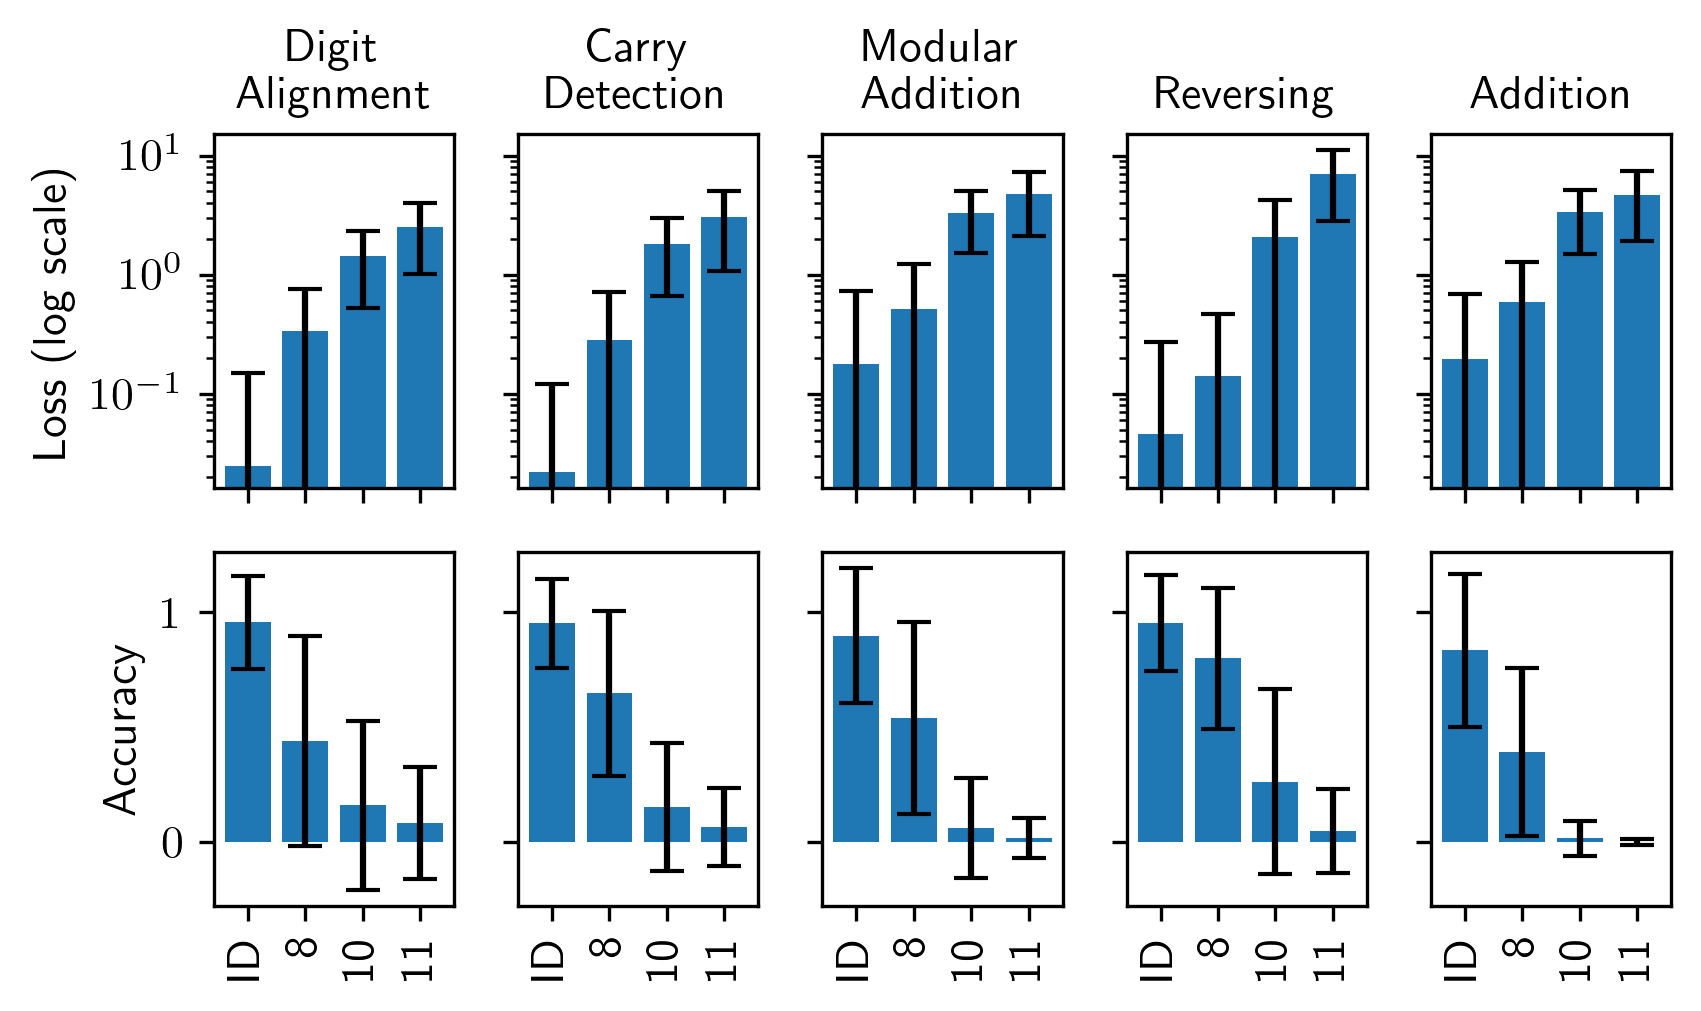
\includegraphics[width=0.9\textwidth]{fig/subtask_difficulty.png}
    \caption{Sub-task difficulty analysis. The bar plots show the mean and standard deviation of test loss (top row) and accuracy (bottom row) across in-distribution (ID) and out-of-distribution (OOD) datasets (8, 10, and 11 digits) and sub-tasks. Loss values across tasks are not directly comparable but can show ID-vs-OOD length deterioration in performance within a task. Based on the accuracy, modular addition and digit alignment are the most difficult sub-tasks, and their performance has the most variability across model sizes as well.}
    \label{fig:subtask_difficulty}
\end{figure}
